\refstepcounter{section}
\section*{Lecture 21: Orbit equation}
In the previous section, we had found the solution to the Einstein metric and in the limit of $GM\to 0$ (i.e, matter-free Universe), the metric reduces to the Minkowski metric. Thus, the Minkowski metric is also a solution of vacuum Einstein field equation.\\[0.2cm] From Eq. \ref{eqn:radial}, we can see that the term $- \frac{3GMl^2}{2m^2r^4}$ is purely an artifact of general relativity and it is an attractive term (comes with minus sign). For $r\to 0$, this term dominates and can cause problem. 
\subsection{Orbit of a Planet in GR}
Since we are considering spherical polar coordinates, we introduce $u = \frac{1}{r}$, from which we get $\dv{u}{\phi} = -\frac{1}{r^2}\dv{r}{\phi}$. The geodesic equations gave us the dynamics of the system, that is, evolution of $r$ and $\phi$ with $\tau$, however, for finding orbits, we need to find $r$ as a function of $\phi$. Then Eq. \ref{eqn:radial} is written as:
\begin{align*}
    \dv{\phi}{\tau} \dv{\phi} \qty( \dv{\phi}{\tau} \dv{r}{\phi}) = -\frac{GM}{r^2} + \frac{l^2}{m^2r^3} - \frac{3GMl^2}{m^3r^4}
\end{align*} 
Recall that we had, $\dv{\phi}{\tau} = \frac{l}{mr^2}$ and $\dv{r}{\phi} = -r^2 \dv{u}{\phi}$, substituting which we obtain:
$$-\frac{l^2u^2}{m^2}\dv[2]{u}{\phi} = -GMu^2 + \frac{l^2 u^3}{m^2} - \frac{3GMl^2}{m^2}u^4$$
Introducing $u_0 = \sfrac{GMm^2}{l^2} = \sfrac{1}{r_0}$, we get a simplified equation:
$$\boxed{\dv[2]{u}{\phi}+u = u_0+3GMu^2}$$
Let us parameterise this solution by $\vep$ such that for $\vep = 0$, we have the Newtonian limit and for $\vep=1$ we obtain the GR solution. Thus, 
\begin{equation}\label{eqn:idk}
    \dv[2]{u}{\phi}+u = u_0+3GM\vep u^2 \quad \longrightarrow \text{solution:} u = u_{\mathrm{N}} + \vep u_{\mathrm{E}}
\end{equation}
$\vartriangleright$ \textbf{Newtonian Solution} $\longrightarrow \vep =0$\\[0.2cm]
Eq. \ref{eqn:idk} becomes the simple harmonic oscillators equation:
$$\frac{\dd^2}{\dd \phi^2}(u-u_0) +(u-u_0)=0$$
whose solution is given by $u(\phi) = u_0 + \SA \cos(\phi-\phi_0)$. We can take $\phi_0=0$. We write this in an alternative form as:
\begin{equation}
    u_N = \frac{1}{r_N} = \frac{1}{r_0}\qty[1+e\cos\phi]
\end{equation}
where $e:=\SA r_0$ is defined to be the \textit{eccentricity} of the orbit. 
$$ \vartriangleright e=0: \text{circular orbit}\quad \vartriangleright e\in (0,1): \text{elliptic orbit}\quad \vartriangleright e=1:\text{parabolic orbit}\quad \vartriangleright e>1: \text{hyperbolic orbit} $$
\begin{figure}[H]
    \centering
    

\tikzset{every picture/.style={line width=0.75pt}} %set default line width to 0.75pt        

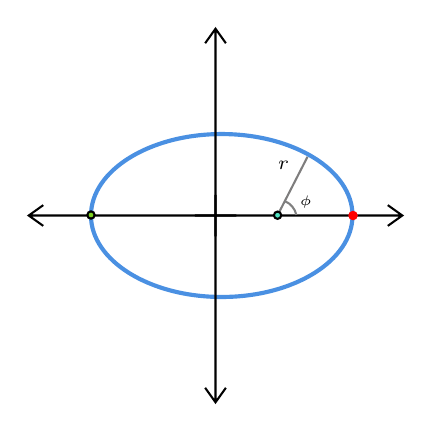
\begin{tikzpicture}[x=0.75pt,y=0.75pt,yscale=-1,xscale=1]
%uncomment if require: \path (0,300); %set diagram left start at 0, and has height of 300

%Straight Lines [id:da5857312553380443] 
\draw [color={rgb, 255:red, 126; green, 125; blue, 125 }  ,draw opacity=1 ]   (289.24,139.76) -- (303.68,111.58) ;
%Shape: Ellipse [id:dp38233645526593374] 
\draw  [color={rgb, 255:red, 74; green, 144; blue, 226 }  ,draw opacity=1 ][line width=1.5]  (199.34,139.9) .. controls (199.34,118.22) and (227.55,100.65) .. (262.34,100.65) .. controls (297.14,100.65) and (325.34,118.22) .. (325.34,139.9) .. controls (325.34,161.58) and (297.14,179.15) .. (262.34,179.15) .. controls (227.55,179.15) and (199.34,161.58) .. (199.34,139.9) -- cycle ;
%Shape: Axis 2D [id:dp300687831343048] 
\draw  (249.34,139.9) -- (349.34,139.9)(259.34,49.9) -- (259.34,149.9) (342.34,134.9) -- (349.34,139.9) -- (342.34,144.9) (254.34,56.9) -- (259.34,49.9) -- (264.34,56.9)  ;
%Shape: Axis 2D [id:dp8884520223518592] 
\draw  (269.34,139.9) -- (169.34,139.9)(259.34,229.9) -- (259.34,129.9) (176.34,144.9) -- (169.34,139.9) -- (176.34,134.9) (264.34,222.9) -- (259.34,229.9) -- (254.34,222.9)  ;
%Shape: Circle [id:dp10092385622889977] 
\draw  [color={rgb, 255:red, 0; green, 0; blue, 0 }  ,draw opacity=1 ][fill={rgb, 255:red, 80; green, 227; blue, 194 }  ,fill opacity=1 ][line width=0.75]  (287.48,139.76) .. controls (287.48,138.79) and (288.27,138) .. (289.24,138) .. controls (290.21,138) and (291,138.79) .. (291,139.76) .. controls (291,140.73) and (290.21,141.52) .. (289.24,141.52) .. controls (288.27,141.52) and (287.48,140.73) .. (287.48,139.76) -- cycle ;
%Shape: Circle [id:dp8729927761800117] 
\draw  [color={rgb, 255:red, 255; green, 0; blue, 0 }  ,draw opacity=1 ][fill={rgb, 255:red, 255; green, 0; blue, 0 }  ,fill opacity=1 ] (323.83,139.9) .. controls (323.83,138.93) and (324.61,138.14) .. (325.58,138.14) .. controls (326.55,138.14) and (327.34,138.93) .. (327.34,139.9) .. controls (327.34,140.87) and (326.55,141.66) .. (325.58,141.66) .. controls (324.61,141.66) and (323.83,140.87) .. (323.83,139.9) -- cycle ;
%Shape: Circle [id:dp11672179474279631] 
\draw  [color={rgb, 255:red, 0; green, 0; blue, 0 }  ,draw opacity=1 ][fill={rgb, 255:red, 126; green, 211; blue, 33 }  ,fill opacity=1 ] (197.58,139.66) .. controls (197.58,138.69) and (198.37,137.9) .. (199.34,137.9) .. controls (200.31,137.9) and (201.1,138.69) .. (201.1,139.66) .. controls (201.1,140.63) and (200.31,141.42) .. (199.34,141.42) .. controls (198.37,141.42) and (197.58,140.63) .. (197.58,139.66) -- cycle ;
%Shape: Arc [id:dp5195085318879069] 
\draw  [draw opacity=0] (292.81,133) .. controls (295.57,134.15) and (297.64,136.61) .. (298.28,139.6) -- (289.24,141.52) -- cycle ; \draw  [color={rgb, 255:red, 128; green, 128; blue, 128 }  ,draw opacity=1 ] (292.81,133) .. controls (295.57,134.15) and (297.64,136.61) .. (298.28,139.6) ;  

% Text Node
\draw (288,112.4) node [anchor=north west][inner sep=0.75pt]  [font=\scriptsize]  {$r$};
% Text Node
\draw (298.46,129.07) node [anchor=north west][inner sep=0.75pt]  [font=\tiny]  {$\phi $};


\end{tikzpicture}
\caption{Elliptical orbit of planet showing the position of perihelion in \textcolor{red}{red}}.
\end{figure}
\noindent
Consider the case of elliptic orbit, with Sun at one of the focus. We consider two special points, called \textit{perihelion} and \textit{aphelion} as the nearest and farthest point to the Sun respectively. Hence to find their position, we need to extremise $u(\phi)$ with respect to $\phi$. Doing this, we obtain:
$$\dv{u}{\phi} = -\frac{e}{r_0}\sin\phi = 0\implies \phi = 2n\pi\ n = 0,1,2\ldots$$
We consider only the perihelion position here. Thus, the Newtonian theory says that perihelion occurs at exactly the same position always. So, after one period of revolution, the planet comes back to the original position (since $\phi = 2n\pi$ all correspond to the same point) however, it was observed that the perihelion shifts gradually. \\[0.2cm]
$\vartriangleright$ \text{GR corrections to the orbit}\\[0.2cm]
Substituting $u=u_{\mathrm{N}} + \vep u_{\mathrm{E}}$ as specified earlier, we have:
\begin{align*}
    \dv[2]{u}{\phi} + u_{\mathrm{N}} + \vep u_{\mathrm{E}} =u_0+ 3GM\vep (u_{\mathrm{N}} + \vep u_{\mathrm{E}})^2   \implies u_0 + \vep \dv[2]{u_{\mathrm{E}}}{\phi} + u_{\mathrm{E}} = u_0 +3GM\vep (u_{\mathrm{N}} + \vep u_{\mathrm{E}})^2 
\end{align*}
Upto $\SO(\vep)$, the RHS is just $3GMu_{\mathrm{N}}^2 \vep$ and hence we have:
$$ \dv[2]{u_{\mathrm{E}}}{\phi} + u_{\mathrm{E}} = 3GMu_{\mathrm{N}}^2 = 3GMu_0^2 (1+e\cos\phi)^2$$
Let us define $u_{\mathrm{E}}^o :=3GMu_0^2$. Now, for many stars, the eccentricity is close to zero, so we can assume $e\ll 1$ which allows us to expand the square term linearly. We get:
\begin{equation}\label{eqn:ue}
    \dv[2]{u_{\mathrm{E}}}{\phi} + u_{\mathrm{E}} = u_{\mathrm{E}}^o(1+2e\cos\phi)
\end{equation}
Assume an ansatz of $u_E =  u_{\mathrm{E}}^o + b\phi \sin\phi$ and note that:
\begin{align*}
    u' = b(\phi \cos\phi + \sin\phi) \\
    u'' = b(2\cos\phi -\phi \sin\phi )
\end{align*}
Substituting this in Eq. \ref{eqn:ue}, we get:
\begin{align*}
    b (2\cos\phi-\phi\sin\phi+\phi\sin\phi)+ u_{\mathrm{E}}^o=  u_{\mathrm{E}}^o(1+2e\cos\phi) \implies \boxed{b=e u_{\mathrm{E}}^o}
\end{align*}
Then upto $\SO(\vep)$ the equation of orbit in GR $(\vep=1)$ becomes:
\begin{equation}\label{eqn:grrad}
    \frac{1}{r(\phi)} =  u_{\mathrm{N}}+  u_{\mathrm{E}} = u_0(1+e\cos\phi) + \qty[3GMu_0^2(1+e\phi\sin\phi)]
\end{equation}
Now, suppose we want to calculate the perihelion for this equation. Ofcourse the perihelion is not going to be some nice expression. However, based on our intuition, we can expect that the shift might not be much from the Newtonian case, hence we assume the perihelion position to be:
$$\phi_n = 2n\pi + \delta \phi$$
Now, we extremise the equation with respect to this $\phi$ and put the above expression for the corrected perihelion. 
\begin{align*}
    \dv{u}{\phi} = -u_0e\sin\phi +3GMu_0^2e\qty(\sin\phi + \phi\cos\phi)\Bigg|_{\phi_n}=0
\end{align*}
Substituting the value of $\phi_n$ and noting that $\sin(2n\pi+x) = x$, we get:
\begin{align*}
    \sin(\delta\phi)(1-3GMu_0) - 3GMu_0(2n\pi+\delta\phi)\cos(\delta\phi) = 0
\end{align*}
Upto $\SO(\delta\phi)$, we obtain $\sin(\delta\phi) \approx \delta \phi$ and $\cos(\delta\phi)\approx 1$. Substituting this above we get:
$$\delta\phi(1-6GMu_0) = 6GMu_0 n\pi \implies \delta\phi =\frac{6GMu_0}{(1-6GMu_0)}n\pi \simeq \frac{6GM^2m^2}{l^2}n\pi$$
Thus, we see that the shift in the perihelion is by a finite angle given by: 
$$\delta\phi = \frac{6GM^2m^2}{l^2}n\pi\longrightarrow \boxed{\Delta\phi = \delta\phi_{n+1} - \delta\phi_n =  \frac{6GM^2m^2}{l^2}}$$
So after one period, the planet does not come back to its original position, indicating the orbit must be changing with time. For Mercury, $\Delta\phi \simeq 43''$ per century which is a really, really minute thing\footnote{ That's what she said \emoji{wink}}, however, the effect is noticeable since we have been collecting data for centuries and also with increasing precision of modern instruments, it is evident. 
\begin{figure}[H]
    \centering
    \includesvg[scale=0.8]{pics/perihelion.svg}
    \caption{Diagram showing the perihelion shift of a planet}
\end{figure}
\subsection{Black Hole}
Note the potential for GR, which has an attractive $\frac{1}{r^3}$ term which dominates for $r\to 0$ and thus, there exists a point of no return, that is, if $r<r_o$, then we cannot come back as $V^{\text{eff}}_{\mathrm{GR}}$ is unbounded from below. 
\begin{figure}[H]
    \centering 
    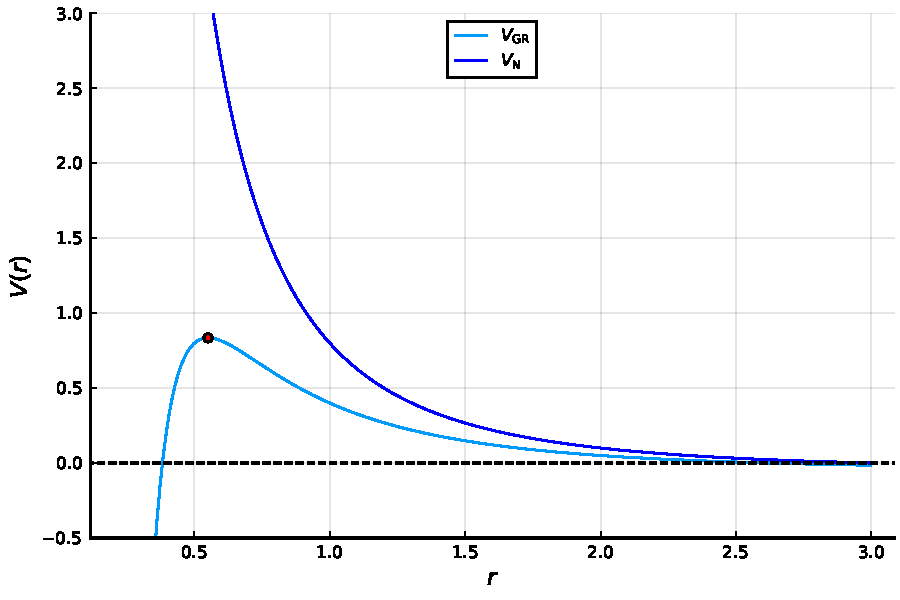
\includegraphics[scale=0.6]{pics/potential.pdf}
    \caption{Comparison between Newtonian and relativisitc effective potentials. The red marker denotes the `point of no return'}
\end{figure}
\noindent
We know that in an inertial frame, photons (light) follows a \textit{null trajectory}, that is, $\dd s^2 = 0$. So suppose we are not in an inertial frame, however due to equivalence principle, we can always go to a locally inertial frame, calculate $\dd s^2$ which will be zero and since $\dd s^2$ is a scalar, it will be zero in all other frames. \\[0.2cm]
Suppose a radial motion of the photon in presence of a point mass $M$ at the origin. Then $\dd\theta =\dd\phi=0$ and $ds^2=0$ and the Schwarzschild metric becomes:
$$0 = \qty(1-\frac{2GM}{r})\dd t^2 +\qty(1-\frac{2GM}{r})^{-1}\dd r^2\implies \dd t^2 = \frac{r^2}{(r-r_s)^2}\dd r^2 $$
$\vartriangleright$ Time taken for light to go from distance $r_o$ to $r_s$ where $r_o<r_s$\\[0.2cm]
The above relation has two roots, however, since we are interested in $r_o<r_s$ case, we take $\dd t = \frac{r}{r_s-r}\dd r$. Integrating this, we get:
\begin{align*}
    \Delta t =\int\limits_{r_o}^{r_s} \frac{r}{r_s-r}\dd r = \int\limits_{r_s}^{r_o} \qty(1 - \frac{r_s}{r_s-r})\dd r = \qty(r + r_s\ln \qty(r_s-r) )\Bigg|_{r_s}^{r_o} = (r_o-r_s) + r_s \qty[\ln(r_s-r_o) - \mathcolor{red}{\lim\limits_{x\to r_s}\ln (r_s - x)}]
\end{align*}
The red term diverges and as a result, the entire expression of $\Delta t$ is divergent. In other words, light would take an infinite amount of time to read $r_s = 2GM$ starting from any arbitrary $r_o<r_s$. Hence, from inside the Schwarzschild radius, even light cannot escape!\\[0.2cm]
We conclude that there is a region of radius $r<r_s$ from where even light cannot escape. The surface $r=r_s$ is called the \textit{event horizon} and such an object is called a \textit{black hole}.\\[0.2cm]
Every galaxy is known to host a black hole at its centre, around which massive stars are observed to rotate. However, since no light can come out of the black hole, we cannot directly observe it. This calculation, even though seem to be a mathematical artifact, has been confirmed through indirect observation of black hole, by using say interferometry of the surroundings of the event horizon (from where light can escape) or gravitational waves. 